\section{Multi-weight} \label{sec:intro}


\begin{table}
\begin{tabular*}{\columnwidth}{|l|p{0.76\columnwidth}|}
\hline
\bf Symbol		& \bf Meaning \\\hline
$G\mathbf{(V,E)}$ 	& A graph with node set $V$ and edge set $E$ \\\hline 
$v_i$			& A node in $V$ \\\hline 
$(v_i,v_j)$		& An edge in $E$ \\\hline 
$W_\omega(v_i,v_j)$	& The edge weight of $(v_i,v_j)$ using weight $\omega \in \mathcal{W}$ \\\hline
$\mathcal{W}$		& Set of possible weight types \\\hline

$Q_{s,t,w}$		& \spath query from node $v_s$ to node $v_t$, using weight $w$\\\hline
$P_{s,t,w}$		& The \spath result of $Q_{s,t,w}$ \\\hline
$|P_{s,t,w}|$		& The size of $P_{s,t,w}$ (in number of nodes) \\\hline
$E_{s,t,w}$		& The expense of executing query $Q_{s,t,w}$ \\\hline
$\chi_{s,t,w}$		& The frequency of a \spath with weight type w \\\hline
$\Psi$ 			& The Cache \\\hline
$\mathfrak{U}(P_{s,t})$	& The set of all subpaths in $P_{s,t}$ \\\hline
$\mathfrak{U}(\Psi)$	& The set of all subpaths of paths in $\Psi$ \\\hline
$\gamma(\Psi)$		& The total benefit of the content in the cache \\\hline

$d_{s,t,w}$		& The \spath distance of a path $P_{s,t,w}$ \\\hline
$\mathfrak{d}_{s,t}$	& $\| t - s \|_2$, the euclidean distance \\\hline

$\mathcal{QL}$		& Query log of search queries \\\hline
\end{tabular*}
\caption{Table of Symbols}
\label{tab:symbols}
\end{table}

% 
% 
% \begin{algorithm}[bht]
% \dontprintsemicolon
% \SetVline
% 
% \SetKwInOut{Input}{input}\SetKwInOut{Output}{output}\SetKw{Return}{return}
% 
% \Input{
% 
% 	$(q,R)$: A Range query\;
% 	$\mathcal{O}$: A set of POI \;
% }
% 
% \Output{
% 
% 	A set \poi $\in \mathcal{O}$ \;
% }
% 
% \funcc{Fair}{(q,R), \mathcal{O}}
% {
%     \ForEach{$o_i \in \mathcal{O} : \mathfrak{d}_{q,o_i} \leq R$}
%     {
%       $candidate_{\mathcal{O}} \leftarrow o_i$ \;
%     }
%     result $\leftarrow$ \naivens((q,R), $candidate_{\mathcal{O}}$) \;
% 
%     \Return{result} \;
% }
% 
% \caption{Fair Algorithm}
% \label{alg:fair}
% \end{algorithm}

\begin{definition}
Let $G(V, E)$ be a graph with a set $V$ of nodes and a set $E$ of edges.
Each node $v_i \in V$ models a road junction. Each edge $(v_i, v_j) \in
E$ models a road segment. The weight (length) of an edge is denoted as $W(v_i, v_j, w)$, where $w \in \mathcal{W}$ is the weight type (length, travel time, scenic value, ect.).
\end{definition}


\begin{equation} \label{eq:upsw}
 \mathfrak{U}_w(\Psi) = \bigcup\limits_{P_{a,b,w} \in \Psi} \mathfrak{U}_w(P_{a,b,d})
\end{equation}

\begin{equation} \label{eq:benefitw}
\gamma_w(\Psi) = \sum\limits_{P_{s,t,w} \in \mathfrak{U}_w(\Psi)} \chi_{s,t,w} \bullet E_{s,t,w}
\end{equation}

\begin{equation} \label{eq:phiw}
\mathfrak{U}_w(P_{a,b,d}) \{ P_{s,t,w} | s \in P_{a,b,d} \wedge t \in P_{a,b,d} \wedge s \neq t \wedge d = w\}
\end{equation}

\begin{equation} \label{eq:chiw}
\chi_{s,t,w} =  \sum\limits_{w \in W } s \in Q_{b,e,w}, t \in Q_{b,e,w}  Q_{b,e,w} \in \mathcal{QL} 
\end{equation}



Equation \ref{eq:phiw} finds all sub-paths of SP $sp$ with weight type $w$. 
Equation \ref{eq:upsw} finds the set of unique paths with weight $w$ from $\Psi$, which is either a path from $a$ to $b$, or a sub-path of such a path. This is the answerable query set of $P_{a,b,d}$.
Equation \ref{eq:benefitw} calculate the benefit of the cache with respect to a specific weight-type.
Equation \ref{eq:chiw} defines the benefit of a path, based on how often we have seen the path, and its subpaths, in the query log $\mathcal{QL}$

Equation \ref{eq:phiw}, \ref{eq:upsw}, and \ref{eq:benefitw} define the existing functions with restriction on $w$. We may however still consider using the old functions.

\begin{definition}{Multi-weight Search}\\
A Multi-weight Search query, denoted by $Q_{s,t,w}$ consist of a source and target vertex $s$ and $t$, plus a weight type $w \in \mathcal{W}$ 
The result of $Q_{s,t,w}$, denoted $SP_{s,t,w}$, is a collection of connected vertices $v_s,\dotsc,v_t$ such that they form a \spath on graph $G\mathbf{(V,E)}$ using weight-type $w \in \mathcal{W}$.
\end{definition}


Using the map in figure \ref{fig:map1} a multi-weight search query, $Q_{v_1,v_2,w}$, can be executed for two different weights, $w_1$ or $w_2$, possibly resulting in two different paths for the same start-/end-nodes, depending on the weight chosen. Table \ref{tab:expsi} shows the \spath $\psi_1$ and $\psi_2$ resulting from the same start-/end-node, but using different weights ($w_1, w_2$).


\begin{definition}{Multi-weight Query Log ($\mathcal{QL_W}$)}\\
A multi-weight search query log $\mathcal{QL_W}$ is a collection of time stamped queries that have been issued by users in the past.
A query is on the form $(s,t,w)$, where $s$ and $t$ is the start- and end-point respectively. $W$ is the weight type to be used when calculating the SP. The full form of the log, $\mathcal{QL_W}$,  is then: $\{(s_0,t_0,w_0),\dots,(s_i,t_i,w_i)\}$. $\chi_{s,t}$ will be the number of sub paths seen, regardless of their weight type, the cost table for $E_{s,t}$ will however need to be maintained for each individual weight type, as each type can incur a different SP.
\end{definition}


\subsection{Cache Structure}

Paths stored as they are in the cache. Instead of using a single inverted list to look up whether the cache can answer a query, we use a collection of inverted lists to keep track of which $Q_{s,t,w}$ can be answered by the cache $\Psi$, for each weight type in $\mathcal{W}$.
Even if a full path can only answer a query for a single weight type, then by using this approach then any sub-path able to answer for more than one weight-type will still be utilized. 

As a path that can answer a SP query for more than one weight type is more valuable then we maintain $\chi_{s,t,\_}$ without regards to the weight type, simply adding up the statistics for each query, for all weight types seen. (This does however not necessarily work very well when we calculate $\chi_{R_i,R_j,w}$ for a pair of regions). 

The map in  fig \ref{fig:map1} depicts a simple road system with 2 different weights on each edge. The first edge weight captures edge length, while the second weight captures the of number of edges traversed, which is why each edge always contributes 1.

Using two example queries, $Q_{v1,v6,\_}, Q_{v1,v5,\_}$, on the map in figure \ref{fig:map1}, we will get the cache items in table \ref{tab:expsi}. Using this we build a inverted list for each weight in order to quickly answer queries (see fig. \ref{fig:wilist}). 
To answer a query $Q_{v_s,v_t,w}$ we use $w$ to first find the relevant inverted list. Afterwards we do 2 look-ups in the inverted list, for $v_s$ \& $v_t$, and do the intersection of the resulting cache items. If the answer is non-empty there is a \spath for $Q_{v_s,v_t,w}$ in the cache.

The same query with different weight can result in different cache items. In table \ref{tab:expsi} the query $Q_{v_1,v_6,X}$ ($X: w_1,w_2$) results in both $\psi_1$ and $\psi_2$ being added to the cache, since the query returns two different paths for weights $w_1$ and $w_2$. It might of cause also be the case that no matter what weight we use, then the \spath is the same. $Q_{v_1,v_5,X}$ show this well, as the \spath does not change for the two weights. One important aspect to notice is that if a full cache item is only valid for a single weight, but a sub path of the \spath is valid for several weights, then this fact will captured in the inverted lists, maximizing the reuse of items in the cache, making them more useful. 



\begin{table}
\begin{tabular}{l|l|l}\hline
$\psi$		& Cache item 			& Weight \\\hline  \hline
$\psi_1:$	& $\{v_1,v_3,v_4,v_5,v_6\}$ 	& ($w_1$)\\\hline
$\psi_2:$	& $\{v_1,v_3,v_6\}$ 		& ($w_2$)\\\hline
$\psi_3:$	& $\{v_1,v_3,v_4,v_5\}$ 	& ($w_1,w_2$)\\\hline
\end{tabular}
\caption{Cache items using queries $Q_{v_1,v_6,X}, Q_{v_1,v_5,X}$ with $X:\{w_1,w_2\}$, covering both weights on the map (fig \ref{fig:map1})}
\label{tab:expsi}
\end{table}


\begin{figure}[hbt]
  \center
        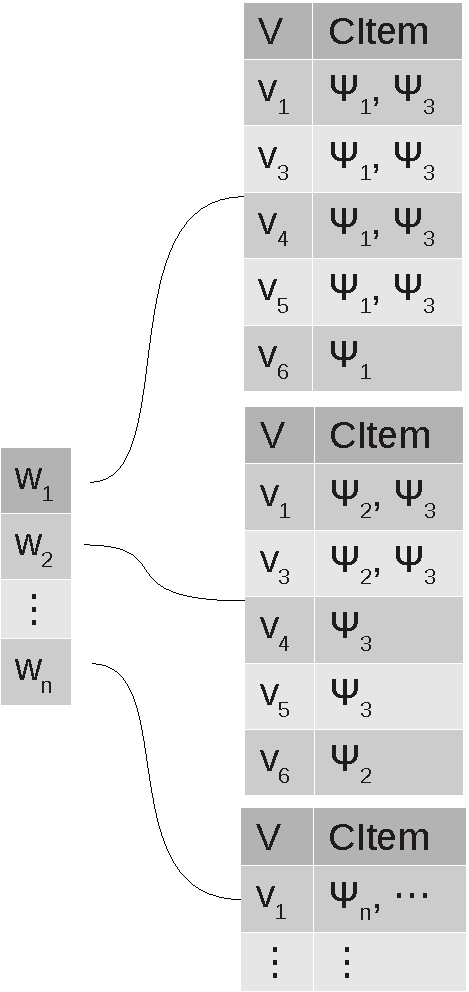
\includegraphics[width=0.3\textwidth]{figures/wilist}
        \caption{Cache structure for inverted lists using map from fig \ref{fig:map1} and cache elements from table \ref{tab:expsi}}
  \label{fig:wilist}
\end{figure}

\begin{figure}[hbt]
  \center
        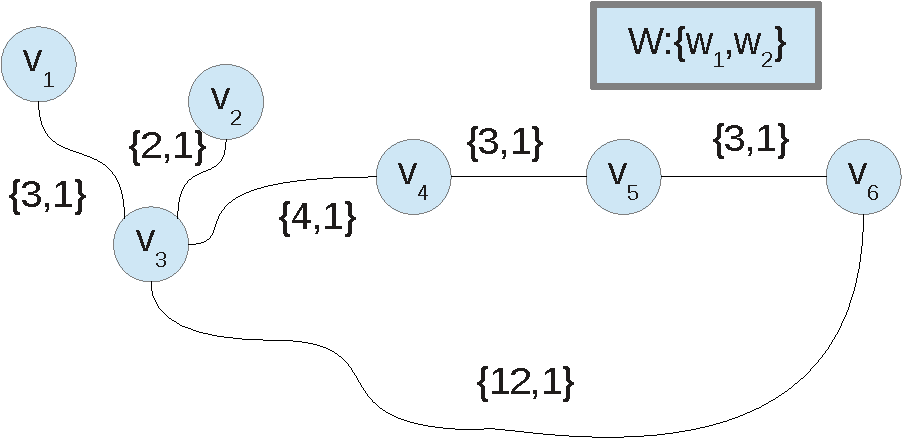
\includegraphics[width=0.4\textwidth]{figures/map1}
        \caption{Map of fig \ref{fig:wilist} and table \ref{tab:expsi}, with set of weights on the edges}
  \label{fig:map1}
\end{figure}


% 
% \begin{tabular}{|l|l|}\hline
% \textbf{V} &	\textbf{Cache Item} \\\hline
% $V_1$	&	$\psi_1, \psi_3$ \\\hline
% $V_3$	&	$\psi_1, \psi_3$ \\\hline
% $V_4$	&	$\psi_1, \psi_3$ \\\hline
% $V_5$	&	$\psi_1, \psi_3$ \\\hline
% $V_6$	&	$\psi_1$ \\\hline
% \end{tabular}
% \vspace{2em}
% 
% \begin{tabular}{|l|l|}\hline
% \textbf{V} &	\textbf{Cache Item} \\\hline
% $V_1$	&	$\psi_2, \psi_3$ \\\hline
% $V_3$	&	$\psi_2, \psi_3$ \\\hline
% $V_4$	&	$\psi_3$ \\\hline
% $V_5$	&	$\psi_3$ \\\hline
% $V_6$	&	$\psi_2$ \\\hline
% \end{tabular}

\section{Minimum Result}


%Intro

%Equations

%Definitions

%explanation

%Figures


\section{Ideas}


%Intro

%Equations

%Definitions

%explanation

%Figures

 \subsection{Sharing Paths}
It might be possible to use several cache items to assist answering a query. There are two ways this seems plausible:
First, by analyzing the map it would be possible to identify junctions such as $v_3$ in \ref{fig:map1}, where any path going to/from $v_1$ or $v_2$ must pass through $v_3$. This would let us do a search in the cache for a partial result, meaning we would have to calculate a smaller \spath. This kind of search would require the \spath algorithm to have a minimum of awareness of whether a junction node could be helpful, though that could be as simple as checking whether the node lies between the x and/or y values of the source and destination of the query.
Second, by analyzing the cache items, and what makes them popular, it might be possible to combine \textit{longer} paths that share a lot of popular nodes, maybe only differing in a \textit{small} set of (not popular) end nodes. By combining the paths we lose the information about some end notes, but we gain a lot of cache space by duplicating less nodes in the cache.
This idea can also be achieved by modifying the way cache items are stored, by compressing the \spaths such that common nodes are stored once with a set of pointer to sets of end nodes. This would effectively achieve the same solution, but it becomes more complicated to query the cache and following pointers around might make the cache slower.

